\documentclass[a4paper,11pt]{scrartcl}
\usepackage[T1]{fontenc}
\usepackage[utf8]{inputenc}
\usepackage{lmodern}
%\usepackage[spanish]{babel}
\usepackage[spanish,es-nodecimaldot]{babel}
\usepackage{mathtools}
\usepackage{amssymb, amsmath, amsbsy}
\usepackage{float}
\usepackage{enumerate}
\usepackage{graphicx}
\usepackage{subfigure}
\usepackage{hyperref}

\title{Cinemática del cuerpo rígido y Cinética del cuerpo rígido}
\subtitle{Cuarto Examen Parcial \\ Equipo 12}
\author{
  Aguilar Enriquez Paul Sebastian\\
  \and
  Benitez Barroso Brandon Raul\\
  \and
  Castillo Herrera Gabriela\\
  \and
  Martinez Vidal Joceline Yadira\\
  \and
  Milán Hernández Maria Fernanda
  }
\date{18 de noviembre del 2016}
\begin{document}

\maketitle

\begin{center}
  Repositorio del documento en GitHub
  \url{https://github.com/penserbjorne/clase-cinematicaydinamica-2017-1}
\end{center}

\textbf{Ejercicio 36} El tambor de freno que se muestra en la  figura~\ref{fig:36_1} está conectado a una rueda más grande que no se muestra en la  figura. El movimiento del disco está gobernado por la ecuación $\theta(t) = At + Bt^{2}$ , donde $\theta$ está en radianes, $t$ en segundos, y las constantes $A$ y $B$ tienen las unidades adecuadas. Determine la velocidad angular cuando $t = t_{0}$ y calcule el número de  revoluciones  que  da  el  tambor  hasta  que  se  detiene.  Evalúa  tus  resultados  cuando $t_{0} = 3 s$, $A = 36 \frac{rad}{s}$ y $B = -1.6 \frac{rad}{s^{2}}$.\\

\begin{figure}[H]
  \centering
  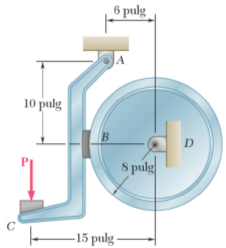
\includegraphics[height=5.5cm]{36_1}
  \caption{Sistema mostrado para el Problema 36.}
  \label{fig:36_1}
\end{figure}

\textbf{Solución:}

\begin{center}

Dado $\theta = 36t - 1.6t^{2}$ radianes.\\
\hfill \break
Obteniendo la velocidad angular\\
\hfill \break
$\omega = \frac{d \theta}{d t} = (36 - 3.2 t) \frac{rad}{s}$\\
\hfill \break
Sustituyendo $t = 3 s$.\\
\hfill \break
$\omega = 36 - (3.2)(3)$\\
\hfill \break
$\omega = 26.4 \frac{rad}{s}$\\
\hfill \break
Cuando la rueda se detiene $\omega = 0$\\
\hfill \break
$0 = 36 - 3.2 t$\\
\hfill \break
Despejamos $t$\\
\hfill \break
$t = 11.25 s$\\
\hfill \break
$\theta = (36)(11.25) - (1.6)(11.25)^{2}$\\
\hfill \break
$\theta = 202.5$ radianes\\
\hfill \break
$\theta = \frac{202.5}{2 \pi}$\\
\begin{equation}
  \left\lbrace
  \begin{array}{l}
    \theta = 32.2 revoluciones
  \end{array}
  \right.
\end{equation}

 
\end{center}

\newpage

\textbf{Ejercicio 39} Para el dispositivo mostrado en la fugura~\ref{fig:39_1}, obtén una expresión para la velocidad angular del engrane $C$ y muestra que ésta es independiente del radio del engrane $B$. Supón que el
engrane $A$ no se mueve (i.e. no gira) y denota la velocidad angular de la barra $ABC$ como $\omega_{0}$.\\

\begin{figure}[H]
  \centering
  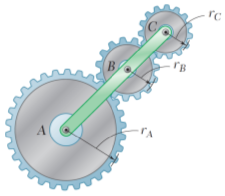
\includegraphics[height=4cm]{39_1}
  \caption{Sistema mostrado para el Problema 39.}
  \label{fig:39_1}
\end{figure}

\textbf{Solución:}

Indicando el punto de contacto entre los engranes A y B como 1, y el punto de contacto entre los engranes B y C como 2 como se muestra en la figura~\ref{fig:39_2}.\\

\begin{figure}[H]
  \centering
  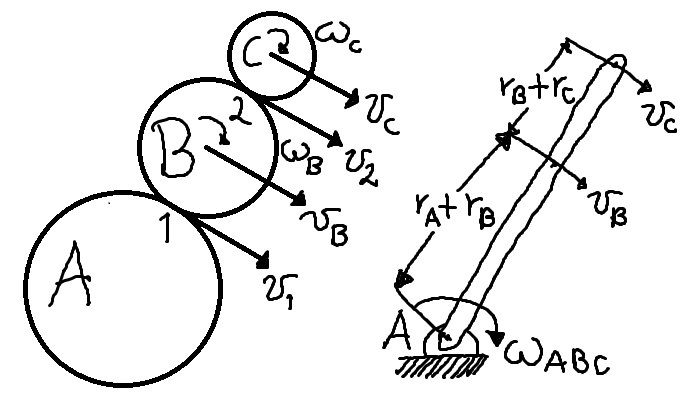
\includegraphics[height=4cm]{39_2}
  \caption{Punto 1 y 2.}
  \label{fig:39_2}
\end{figure}

\begin{center}
Barra $ABC$: \\
\hfill \break
$\omega_{ABC} = \omega_{ABC}$\\
\hfill \break
Considerando el sentido de giro de $\omega_{ABC}$ como se muestra en el diagrama:\\
\hfill \break
$V_A = 0$\\
\hfill \break
$V_B = (r_A + r_B) \omega_{ABC}$\\
\hfill \break
$V_C = (r_A + 2r_B + r_C) \omega_{ABC}$\\
\hfill \break
En el engrane A:\\
\hfill \break
$\omega_A = 0$, $V_A = 0$, $V_1 = 0$\\
\hfill \break
En el engrane B:\\
\hfill \break
$V_1 = V_B - r_B \omega_B = 0$\\
\hfill \break
$(r_A + r_B) \omega_{ABC} - r_B \omega_B = 0$\\
\hfill \break
$\omega_B = ( \frac{ r_A + r_B}{r_B} ) \omega_{ABC}$\\
\hfill \break
$V_2 = V_B + r_B \omega_B$\\
\hfill \break
$V_2 = 2(r_A + r_B) \omega_{ABC}$\\
\hfill \break
En el engrane C:\\
\hfill \break
$V_2 = V_C - r_C \omega_C$\\
\hfill \break
$2(r_A + r_B) \omega_{ABC} = (r_A + 2r_B + r_C) \omega_{ABC} - r_C \omega_C$\\
\hfill \break
$\omega_C = (r_A - r_C) \omega_{ABC} = -r_C \omega_C$\\
\begin{equation*}
  \left\lbrace
  \begin{array}{l}
    \omega_C = (1 - \frac{r_A}{r_C}) \omega_{ABC}
  \end{array}
  \right.
\end{equation*}


\end{center}

\newpage

\textbf{Ejercicio 44} El tambor de freno, de $8 in$ de radio, está unido a un volante más grande que no se muestra en la figura~\ref{fig:44_1}. El momento de inercia de la masa total del tambor y del volante es
de $14 lb * ft * s^2$ y el coeficiente de frcción cinética entre el tambor y la zapata del freno es de $0.35$. Si la velocidad angular del volante es de $360 rpm$ en el sentido de las manecillas del reloj cuando se aplica una fuerza $\hat{P}$ de $75 lb$ de magnitud al pedal $C$, determine el número de revoluciones realizadas por el volante antes de detenerse.\\

\begin{figure}[H]
  \centering
  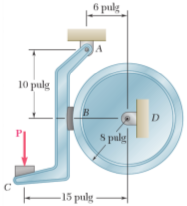
\includegraphics[height=4cm]{44_1}
  \caption{Diagrama correspondiente al Problema 44.}
  \label{fig:44_1}
\end{figure}

\textbf{Solución:}

\begin{center}

Empezamos notando que, al aplicar la fuerza $\hat{P}$ sobre el freno, se llega a un equilibrio en las torcas con respecto al punto A, utilizando la regla de la mano derecha y tomando en cuenta el sentido del giro del tambor\\
\hfill \break
$\Sigma \hat{\tau}_A = \hat{0} \Rightarrow -\hat{r}_N \times \hat{N} - \hat{r}_f \times \hat{F} + \hat{r}_P \times \hat{P} = \hat{0}$\\
\hfill \break
donde $\hat{N}$ es la fuerza normal debida al tambor y $\hat{F}$ es la fuerza de fricción debida al roce del tambor con la zapata. Notando que cada ángulo que forma cada fuerza con su respectivo brazo de palanca, reescribimos la ecuacion como:\\
\hfill \break
$-r_N N - r_F F + r_P P = 0$\\
\hfill \break
pero, recordando que la magnitud de la fuerza de friccion es $F = fN$, donde $f$ es el coeficiente de fricción cinética, resolvemos para la magnitud de la friccion y obtenemos:\\
\hfill \break
$F = \frac{f r_p}{r_N + f r_F} P$\\
\hfill \break
Ahora, en el sistema del tambor, tomando en cuenta las torcas que se ejercen debido a la fricción y a la normal (con respecto al centro D y usando nuevamente la mano de la regla derecha), podemos escribir:\\
\hfill \break
$\Sigma \hat{\tau}_D = I \hat{\alpha} \Rightarrow \hat{r}_D \times \hat{F} = I \hat{\alpha}$\\
\hfill \break
donde $I$ es el momento de inercia del tambor y el volante, $\hat{\alpha}$ es su aceleración angular y $r_D$ es el radio del disco. Nótese que la torca debida a la normal se anula ya que la normal es la clineal con su brazo de palanza. Así, obtenemos la ecuación diferencial de la dinámica del tambor-volante\\
\hfill \break
$\alpha = \frac{d \omega (\theta)}{d t} = - \frac{r_D F}{I} < 0$ i.e. el sistema se desacelera\\
\hfill \break
donde se ha supuesto que, tanto $\alpha$ como $\omega$ son funciones del angulo $\theta$. Por tanto, utilizando la regla de la cadena $\alpha = \omega \frac{d \omega}{d \theta}$, por lo que \\
\hfill \break
$\int_{\omega_0}^{0} \omega d \omega = \alpha \int_{0}^{\theta} d \theta' \Rightarrow \theta \alpha = \left.\frac{\omega^2}{2}\right\vert_{\omega_0}^{0} \Rightarrow \theta = \frac{{\omega_0}^2}{2 \alpha}$\\
\hfill \break
donde se integra desde la velocidad angular del tambor-volante justo antes de que se aplique el freno $\omega_0$ hasta que éste se detiene, que según la ecuacion de $\alpha$, la aceleración angular es constante. Así, tomando los valores dados inicialmente y usando la ecuación de $F$, la ultima ecuacion obtenida implica finalmente que\\
\hfill \break
\begin{equation*}
  \left\lbrace
  \begin{array}{l}
  \theta = \frac{I {\omega_0}^2 (r_N + f r_F)}{2 f r_D r_P P} = \frac{1712}{25} {\pi}^2 rad = \frac{856}{25} \pi rev
  \end{array}
  \right.
\end{equation*}
\end{center}

\newpage

\textbf{Ejercicio 45} Un neumético de radio $r$ y radio de giro centroidal $\hat{k}$ se suelta desde el reposo sobre una pendiente y rueda sin deslizarse como se muestra en la  figura~\ref{fig:45_1}. Obtenga una expresión para la aceleración del centro del neumático en términos de $r$, $\hat{k}$, $\beta$ y $g$.\\

\begin{figure}[H]
  \centering
  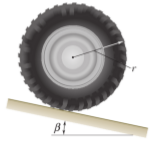
\includegraphics[height=4cm]{45_1}
  \caption{Diagrama correspondiente al Problema 45.}
  \label{fig:45_1}
\end{figure}

\textbf{Solución:}

\begin{center}

Partiendo de lo siguiente:\\
\hfill \break
Particular:\\
$I_P = mr^2$\\
\hfill \break
Barra:\\
$I_{cm} = \frac{1}{12} ML^2$\\
\hfill \break
$I_{z'} = \frac{1}{3} ML^2$\\
\hfill \break
Disco:\\
$I_{cm} = \frac{1}{2} MR^2$\\
\hfill \break
$I_{z'} = \frac{3}{2} MR^2$\\
\hfill \break
Esfera Solida:\\
$I_{cm} = \frac{2}{5} MR^2$\\
\hfill \break
Sabemos que:\\
\hfill \break
$I = n M L^2 = M R^2$\\
\hfill \break
$k = \sqrt{n} L$\\
\hfill \break
$\Sigma \hat{\tau} = I_{eff} \hat{\alpha} = m \hat{r} \times a_0 + I \hat{\alpha}$\\
\hfill \break
$\hat{a} = \frac{d \hat{v}}{d t} = \Rightarrow \hat{r}\times \hat{a} = m r^2 \hat{\alpha}$\\
\hfill \break
$\hat{r} \times \hat{\omega} = m \hat{r} \times \hat{a}_0 + I \hat{\alpha}$\\
\hfill \break
$-r\omega sen(\beta) = - m r a_0 - I \frac{a_0}{r}$\\
\hfill \break
Sabiendo que:\\
\hfill \break
$V = \omega r$, $a_0 = \alpha r$, $I = m \hat{k}^2$ y $\omega = m g$\\
\hfill \break
Sistituyendo y despejando:\\
\hfill \break
$a_0 = \frac{r \omega sen(\beta)}{mr - \frac{I}{r}} = \frac{r \omega sen(\beta)}{mr + \frac{m \hat{k}^2}{r}} = \frac{r g sen(\beta)}{r + \frac{\hat{k}^2}{r}}$\\
\hfill \break
\begin{equation*}
  \left\lbrace
  \begin{array}{l}
   \frac{r^2 g sen(\beta)}{r^2 + \hat{k}^2}
  \end{array}
  \right.
\end{equation*}

\end{center}

\end{document}
